%%%%%%%%%%%%%%%%%%%%%%%%%%%%%%%%%%%%%%%%%%%%%%%%%%%%%%%%%
% French Regional Conference on Complex Systems
% May 29-31, 2024, Montpellier, France
%
%
% Please follow these general guidelines:
% (1) Compile with pdflatex
% (2) Do not alter the style commands.
% (3) Do not add newcommand, newenviroments, etc. 
%%%%%%%%%%%%%%%%%%%%%%%%%%%%%%%%%%%%%%%%%%%%%%%%%%%%%%%%%
\documentclass{frccs2024}

\begin{document}

% Title and running title (short title) to be used as header
\title{Title of the talk}
\titlerunning{Include short title (up to 50 characters)}

% Authors and running list of authors to be used as header
% Author names must be included as: "Name Surname"
% Author names for running titles must be specified as:
% For one author: N. Surname
% For two authors: N1. Surname1 and N2. Surname2
% For more than two authors: N1. Surname \emph{et al.}
% Use \speaker for the presenter.

\authors{\speaker{Name1 Surname1$^{1}$}, Name2 Surname2$^2$ and Name3 Surname3$^1$}
\authorsrunning{N. Surname1 \emph{et al.}}

% Full address for correspondence and e-mail of all authors
\addresses{%
$^1$ Common affiliation of (first and third) authors ; first.author@email, third.author@email.\\ 
$^2$ Distinct affiliation of second author ; second.author@email
}

% Abstract (at most 500 signs)
\abstract{A scientific abstract is a concise summary of a research paper, typically not exceeding 500 characters. It should briefly introduce the research question, methods employed, key findings, and their significance. Avoiding jargon, it must provide enough context for readers to understand the study's importance and conclusions. Clear and structured, it serves as a snapshot, guiding readers in deciding whether to delve deeper into the full paper.}

% Keywords (at most 5)
\keywords{Keyword1; Keyword2. Include up to five keywords separated by semi--colons starting with capital letters.}

\maketitle
\section{Formatting Tips}

The \texttt{frccs2024} document class provides \LaTeX{} styles for the FRCCS 2024 Conference. The class depends on several packages to format the document. Please avoid modifying the format or including packages that alter fonts, sizes, margins, or alignments. Here are some typesetting guidelines.

\subsection{Citations and References}

To create citations and references, use the \texttt{thebibliography} environment or utilize an external tool like \texttt{bibtex} with the \texttt{plain} bibliography style. Cite references with the \texttt{cite} command (e.g., \texttt{\textbackslash cite\{lamport1994latex\}}) \cite{lamport1994latex}. 

\subsection{Figures and Images}

For figures and images, employ the \texttt{figure} environment with a \texttt{\textbackslash caption} and a \texttt{\textbackslash label} command. For instance:

\begin{verbatim}
\begin{figure}[ht]
    \centering
    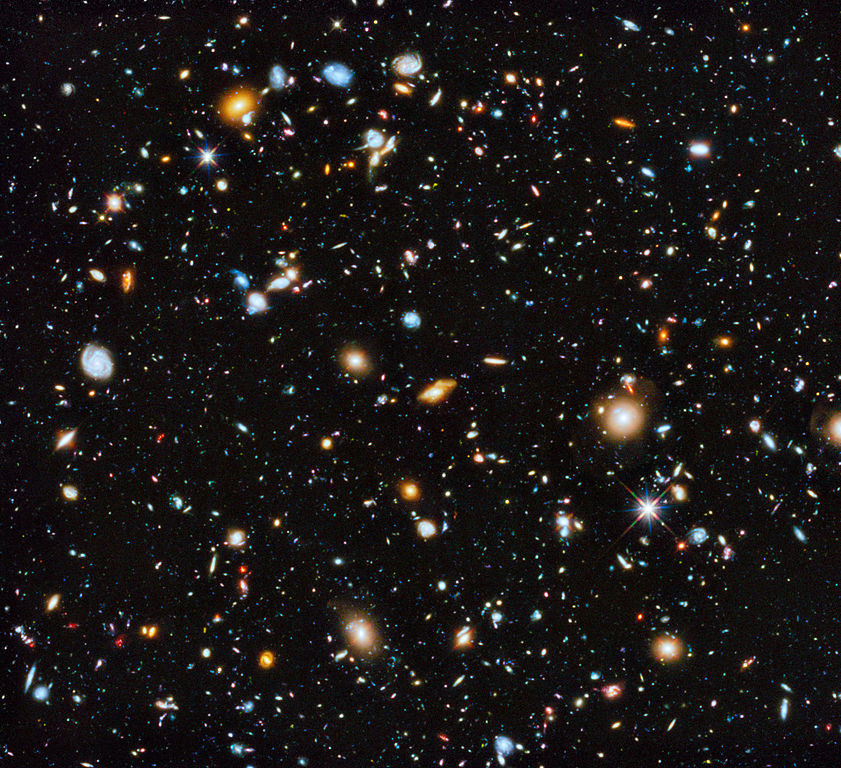
\includegraphics[width=0.7\linewidth]{hubble.jpg}
    \caption{Hubble Ultra Deep Field...}
    \label{fig:hubble}
\end{figure}
\end{verbatim}

Use the \texttt{\textbackslash includegraphics} command to insert images, specifying the size proportionally to \texttt{\textbackslash linewidth}.


\begin{figure}[ht]
    \centering
    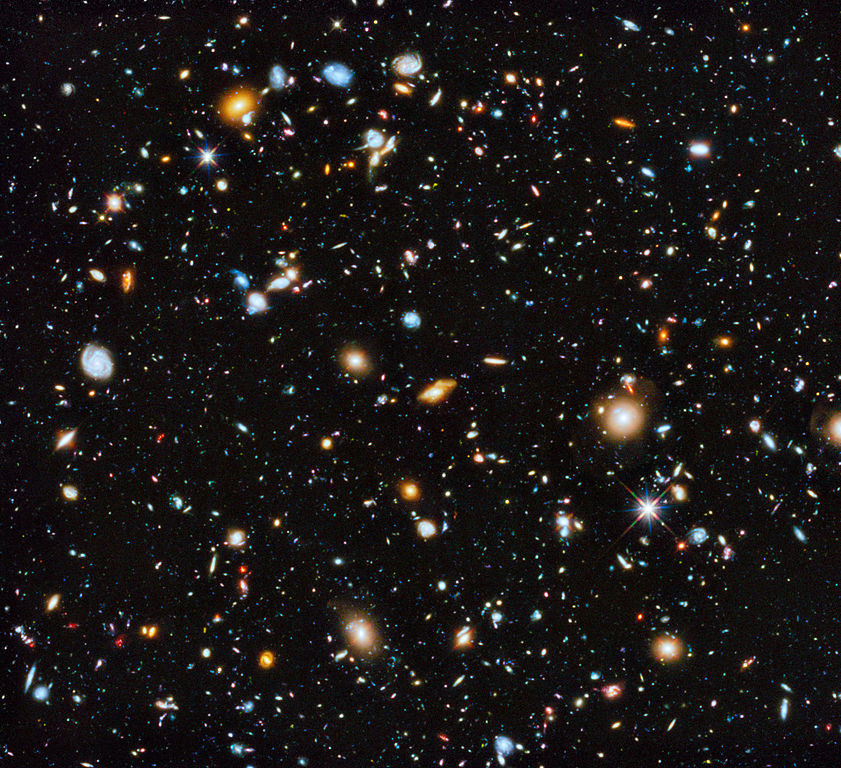
\includegraphics[width=0.6\linewidth]{hubble.jpg}
    \caption{The Ultraviolet Coverage of the Hubble Ultra Deep Field (UVUDF) project. Credit: NASA, ESA, H. Teplitz and M. Rafelski (IPAC/Caltech), A. Koekemoer (STScI), R. Windhorst (Arizona State University), and Z. Levay (STScI).}
    \label{fig:hubble}
\end{figure}


Use the \texttt{ref} command (e.g. \texttt{\textbackslash ref\{fig:hubble\}} ) to refer to Figure \ref{fig:hubble}. 


\subsection{Tables}

Tables should be centered floats within the \texttt{table} environment, featuring a caption and a label atop the table. Separate headers from the body with a double line. Avoid excessive bars and lines around the table. For example:

\begin{verbatim}
\begin{table}[ht]
\caption{A Simple Table}
\label{tab:simple}
\begin{center}
\begin{tabular}{ c | c | c }
 Col1 & Col2 & Col3  \\
 \hline\hline
 1 & 6 & 87837  \\
 \hline
 5 & 88 & 788  \\
\end{tabular}
\end{center}
\end{table}
\end{verbatim}

\begin{table}[ht]
\caption{A Simple Table}\label{tab:simple}
\begin{center}
\begin{tabular}{ c | c | c | c } 

 Col1 & Col2 & Col2 & Col3 \\ 
 \hline\hline 
 1 & 6 & 87837 & 787 \\ 
 \hline
 2 & 7 & 78 & 5415 \\
 \hline
 3 & 545 & $1/778$ & $n log(n)$ \\
 \hline
 4 & 545 & $\sqrt{234}$ & 7560 \\
 \hline
 5 & 88 & 788 & 6344 \\
\end{tabular}
\end{center}
\end{table}

Refer to Table \ref{tab:simple} using the \texttt{ref} command (e.g., \texttt{\textbackslash ref\{tab:simple\}}).

Combining rows and columns can be achieved with the \texttt{multirow} package, while multi-page tables should refer to the \texttt{longtable} packages. 

\section{Second Section}

Vivamus eu tortor felis. Nam justo ipsum, ultrices quis ante quis, auctor mattis tellus. Interdum et malesuada fames ac ante ipsum primis in faucibus. Sed nec pellentesque lectus, at egestas eros. Praesent laoreet neque at velit scelerisque lacinia. Vivamus vitae est mi. Mauris aliquam metus et purus blandit, eget dapibus lectus vestibulum. Quisque mollis cursus iaculis. Curabitur ultricies non arcu eu placerat. Nunc aliquet vitae purus vitae bibendum. Duis varius enim quis elit accumsan feugiat. Donec hendrerit, quam id molestie vehicula, eros metus fringilla lorem, vel sodales ante risus nec nulla. Curabitur suscipit finibus purus, id rutrum arcu dapibus eu. Suspendisse dictum id sapien sed ultricies.

Aenean efficitur lacus convallis augue scelerisque consequat. Lorem ipsum dolor sit amet, consectetur adipiscing elit. Mauris vitae nulla vitae nunc feugiat euismod non ac ante. Curabitur quis viverra libero. Mauris non faucibus massa. Maecenas at tristique felis. In feugiat nunc a sapien placerat, ut aliquet enim fringilla. Aliquam vel porta nunc, nec consectetur tortor. Etiam suscipit sapien dignissim justo molestie egestas.

Duis ipsum lorem, malesuada eget urna vitae, porttitor luctus sem. Phasellus aliquet magna in massa congue, at fermentum mauris semper. Phasellus sit amet nisl eget ipsum rhoncus auctor vel in urna. Quisque egestas dolor sit amet ligula rhoncus, ut fermentum sapien euismod. Donec eget libero lobortis, bibendum magna venenatis, tincidunt elit. Pellentesque convallis, elit eu gravida dapibus, ex felis maximus urna, id luctus ante tellus non nibh. Mauris congue tincidunt blandit. Fusce posuere ullamcorper elit, eu accumsan purus molestie non. Curabitur sed aliquet justo. Proin at rhoncus mauris. Vivamus eu lacinia dolor, vel fringilla sem. Proin tincidunt justo in molestie condimentum. Integer ut massa in enim consequat bibendum eu quis nibh. Sed iaculis sit amet orci eu euismod.


Nam pellentesque maximus turpis. Aenean lobortis mattis faucibus. Proin et justo a turpis tempus semper dictum ut leo. Vestibulum nec euismod felis, rutrum luctus felis. Proin finibus purus non magna vehicula, vitae commodo sem faucibus. Morbi fringilla congue dui id gravida. Etiam vitae elementum quam. Etiam pretium porttitor purus eu facilisis. Sed non augue ut mauris interdum gravida a convallis nibh. Cras urna sem, accumsan sed feugiat in, cursus eget eros. Etiam auctor ultrices ipsum, eget aliquam turpis convallis eget. Class aptent taciti sociosqu ad litora torquent per conubia nostra, per inceptos himenaeos. Mauris eget orci efficitur, commodo enim facilisis, pharetra ligula. Maecenas mi felis, volutpat eu ultricies eu, bibendum eget orci. Aliquam convallis enim urna, vitae sollicitudin nulla consequat non.

%%%%%%% References 
% Use : 
% (1) the `thebibliography` environment with a list of `bibiten` commands, 
% or 
% (2) the `bibliography` with bibbex and a .bib file

% (1) `thebibliography` environment
%\begin{thebibliography}{99}
%\bibitem{knuth1986texbook} 
%D. E. Knuth. \emph{The \TeX{} Book}. Computers \& typesetting. Addison-Wesley, 1986.
%\bibitem{lamport1994latex}
%L. Lamport. \emph{LATEX: A Document Preparation System : User’s Guide and Reference Manual}. Addison-Wesley series on Tools and Techniques for Computer Typesetting. Addison-Wesley, 1994.
%\end{thebibliography}
%%%

% (2) the `bibliography` command with a .bib file
\nocite{*}
\bibliography{biblio.bib}


\end{document}



